\section{Neutronic Constraints}

A valid reactor design must meet certain neutronics constraints. The main
neutronics constraint is reactivity. The reactor must be able to sustain a chain
reaction from startup, to the final second of the 10 year lifetime. End of Life
(EOL) reactivity was the target metric for the neutronic design of the core. It
was important to determine which reactor parameters had the strongest impact on
EOL \keff. An n-dimensional sampling was performed to explore EOL \keff
dependence on various reactor parameters.

\subsection{Neutronics Parameters}
Homogeneous MCNP6.1 depletion models were used to analyze the EOL \keff response
to neutronics parameters (predictors). The core region was homogenized and
surrounded by a graphite reflector. A large set of 5-dimensional predictors and
EOL \keff results was produced to investigate the neutronics parameter space.
These predictors and their results helped develop an understanding of the
reactor response to important design and operational parameters. High Throughput
Computing capabilities at UW were used to perform 3901 depletion calculations
with MCNP6.1. Each model represents a unique sampling in every dimension using
the Latin Hypercube Sampling (LHS) technique. The LHS technique ensured even
sampling for every dimension. The sampled and fixed dimensions/parameters are
shown in Table \ref{tab:lhs_sweep_vars}.

\begin{table}[h]
  \centering
  \caption{Homogeneous Geometry and Depletion Parameters}
  \begin{tabular}{ll}
    \toprule
     Core Radius                		   & 10 - 50 [cm] \\
     Reflector Thickness				   & 15 [cm]\\
     Core Aspect Ratio					   & 1 [-] \\
     Coolant Channel Radius                & 0.5 - 1 [cm] \\
     Fuel Pitch to Coolant Channel D.      & 1.1-1.6 [-]\\
     Fuel Enrichment 					   & 20\% - 90\% $^{235}$U\\
     Thermal Power						   & 80-200 [kW]\\
     Fuel Temp  						   & 300 [K]\\
     Reactor Physics Code, Data			   & MCNP6.1, ENDF-7.2
  \end{tabular}
  \label{tab:lhs_sweep_vars}
\end{table}

\subsection{Neutronics Sampling Results}
The target metric for the neutronics sampling was an EOL \keff equal to one. In
order to determine the dependence of EOL \keff on each swept parameter in Table
\ref{tab:lhs_sweep_vars}, EOL \keff was plotted against the parameters.

\subsubsection{Thermal Power}
Initially, the result of greatest interest was the mass dependence on thermal
power because thermal power was the coupling parameter with the power cycle.
Figure \ref{fig:eol_keff_vs_power} shows the relationship between thermal power
and EOL \keff.

\begin{figure}[h]
    \centering
    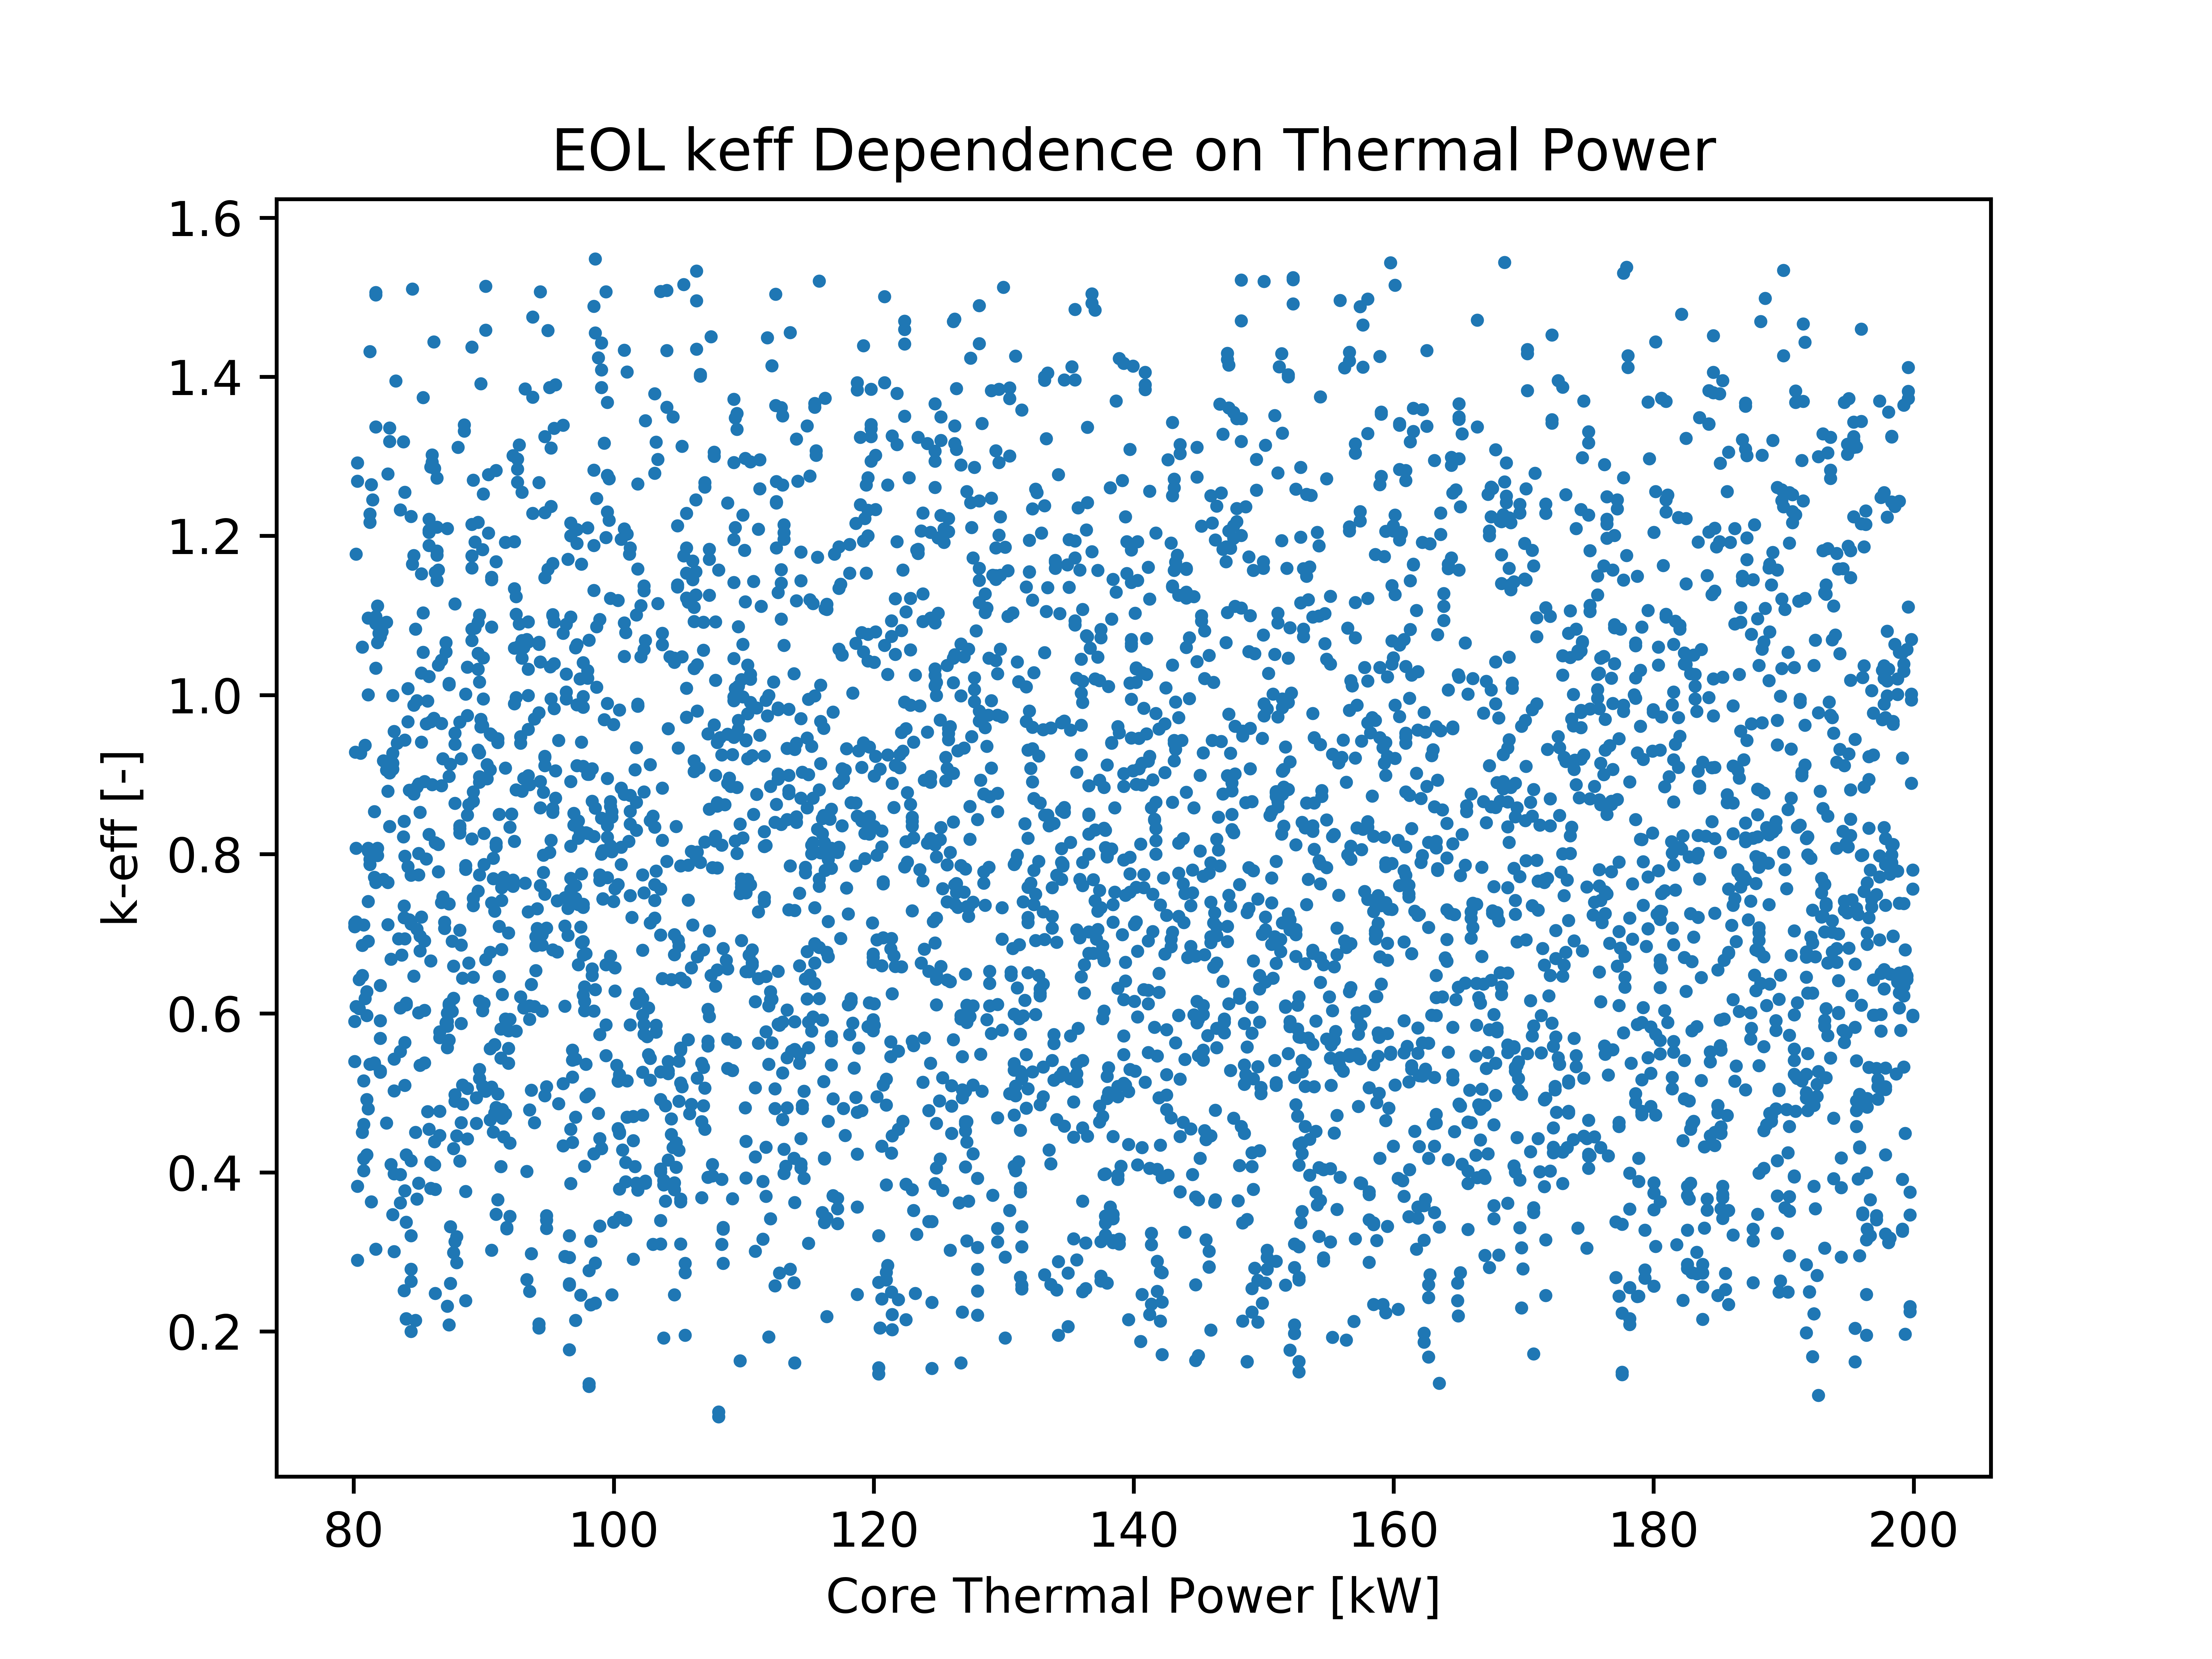
\includegraphics[width=3in]{nd_sweeps/keff_vs_power.png}
\caption{EOL \keff Power Dependence}
\label{fig:eol_keff_vs_power}
\end{figure}

As shown in Figure \ref{fig:eol_keff_vs_power}, EOL \keff is independent of core
thermal power. This result is not surprising considering the depletion rates in
the core. Assuming 1 MWd/gU is an achievable burnup, the reactor depletes
approximately 1000 kg of uranium at 200 kW of thermal power. The depletion mass
of uranium is negligigle compared to the mass of uranium required for the
reactor to be critical at BOL. Thermal power is not a strong predictor of EOL
criticality.

\subsubsection{Uranium 235 Mass}

